% Options for packages loaded elsewhere
\PassOptionsToPackage{unicode}{hyperref}
\PassOptionsToPackage{hyphens}{url}
%
\documentclass[
]{article}
\usepackage{lmodern}
\usepackage{amsmath}
\usepackage{ifxetex,ifluatex}
\ifnum 0\ifxetex 1\fi\ifluatex 1\fi=0 % if pdftex
  \usepackage[T1]{fontenc}
  \usepackage[utf8]{inputenc}
  \usepackage{textcomp} % provide euro and other symbols
  \usepackage{amssymb}
\else % if luatex or xetex
  \usepackage{unicode-math}
  \defaultfontfeatures{Scale=MatchLowercase}
  \defaultfontfeatures[\rmfamily]{Ligatures=TeX,Scale=1}
\fi
% Use upquote if available, for straight quotes in verbatim environments
\IfFileExists{upquote.sty}{\usepackage{upquote}}{}
\IfFileExists{microtype.sty}{% use microtype if available
  \usepackage[]{microtype}
  \UseMicrotypeSet[protrusion]{basicmath} % disable protrusion for tt fonts
}{}
\makeatletter
\@ifundefined{KOMAClassName}{% if non-KOMA class
  \IfFileExists{parskip.sty}{%
    \usepackage{parskip}
  }{% else
    \setlength{\parindent}{0pt}
    \setlength{\parskip}{6pt plus 2pt minus 1pt}}
}{% if KOMA class
  \KOMAoptions{parskip=half}}
\makeatother
\usepackage{xcolor}
\IfFileExists{xurl.sty}{\usepackage{xurl}}{} % add URL line breaks if available
\IfFileExists{bookmark.sty}{\usepackage{bookmark}}{\usepackage{hyperref}}
\hypersetup{
  pdftitle={Natureza das Transformações no Setor de Produção de Bens Culturais},
  pdfauthor={Alberson da Silva Miranda},
  hidelinks,
  pdfcreator={LaTeX via pandoc}}
\urlstyle{same} % disable monospaced font for URLs
\usepackage[margin=1in]{geometry}
\usepackage{graphicx}
\makeatletter
\def\maxwidth{\ifdim\Gin@nat@width>\linewidth\linewidth\else\Gin@nat@width\fi}
\def\maxheight{\ifdim\Gin@nat@height>\textheight\textheight\else\Gin@nat@height\fi}
\makeatother
% Scale images if necessary, so that they will not overflow the page
% margins by default, and it is still possible to overwrite the defaults
% using explicit options in \includegraphics[width, height, ...]{}
\setkeys{Gin}{width=\maxwidth,height=\maxheight,keepaspectratio}
% Set default figure placement to htbp
\makeatletter
\def\fps@figure{htbp}
\makeatother
\setlength{\emergencystretch}{3em} % prevent overfull lines
\providecommand{\tightlist}{%
  \setlength{\itemsep}{0pt}\setlength{\parskip}{0pt}}
\setcounter{secnumdepth}{5}
\usepackage{quoting, setspace}

\newenvironment{citacao}
    {\begin{quoting}[rightmargin=0cm,leftmargin=4cm]
    \begin{singlespace}
    \footnotesize
    }
    {\end{singlespace}
    \end{quoting}
    }
    
\ifluatex
  \usepackage{selnolig}  % disable illegal ligatures
\fi
\usepackage[]{natbib}
\bibliographystyle{apalike}

\title{Natureza das Transformações no Setor de Produção de Bens
Culturais}
\author{Alberson da Silva Miranda}
\date{2022-05-31}

\begin{document}
\maketitle

\hypertarget{introduuxe7uxe3o}{%
\section*{INTRODUÇÃO}\label{introduuxe7uxe3o}}
\addcontentsline{toc}{section}{INTRODUÇÃO}

A economia está inserida na esfera social e, portanto, determinada por
fenômenos sociais. Suas regras, normas e relações estão, por essa razão,
sujeitas à geografia, tempo e estruturas de
poder\footnote{Aqui me refiro às instituições que ora determinaram o \textit{ethos} vigente, como a igreja, aristrocacia ou o capital, por exemplo.}.
Isso implica que seu funcionamento em raras ocasiões --- ou em nenhuma
--- poderá ser explicado por \emph{leis da natureza}, que, por
definição, são imutáveis. E no caso dos bens culturais, há evidências de
transformações profundas nos últimos anos.

Neste estudo, {[}\ldots{]}

\hypertarget{fatos-estilizados-da-induxfastria-cultural-nos-anos-2000}{%
\section{FATOS ESTILIZADOS DA INDÚSTRIA CULTURAL NOS ANOS
2000}\label{fatos-estilizados-da-induxfastria-cultural-nos-anos-2000}}

A indústria cultural tem sofrido mudanças profundas nos últimos 20 anos.
Avanços tecnológicos, estrutura de receita e oligopolização são alguns
dos fatores que afetaram várias dimensões do setor de bens culturais ---
cinematográfica, televisiva, musical, literária e até mesmo de jogos
eletrônicos.

Dentre os fatores tecnológicos, a sequência de inovações nas mídias que
culminaram no advento do \emph{streaming} são de fundamental
importância. No audiovisual, enquanto as mídias físicas --- fitas
cassetes e vinis --- dominavam o mercado e a internet ainda não era
largamente disponível, a pirataria era menos viável e de menor
qualidade. Em 2001, 98\% da receita da indústria da música gravada era
oriunda das mídias físicas. Com a introdução do \emph{compact disk} ---
o CD---, a propagação da internet e a popularização de computadores com
\emph{drive} de disco, se torna simples a cópia física e digital da
música gravada, dando ímpeto à pirataria. É nesse momento que sites
especializados e tecnologias de compartilhamento, como o \emph{torrent}
e o P2P\footnote{Limeware, Kazaa e eMule, por exemplo.}, surgem. Lançado
o iPod, em 2001, a transição para a mídia digital alcança também os
reprodutores móveis, tornando obsoleto o \emph{discman} e concluindo a
transição da mídia analógica para a digital \citet{commons}.

\begin{figure}
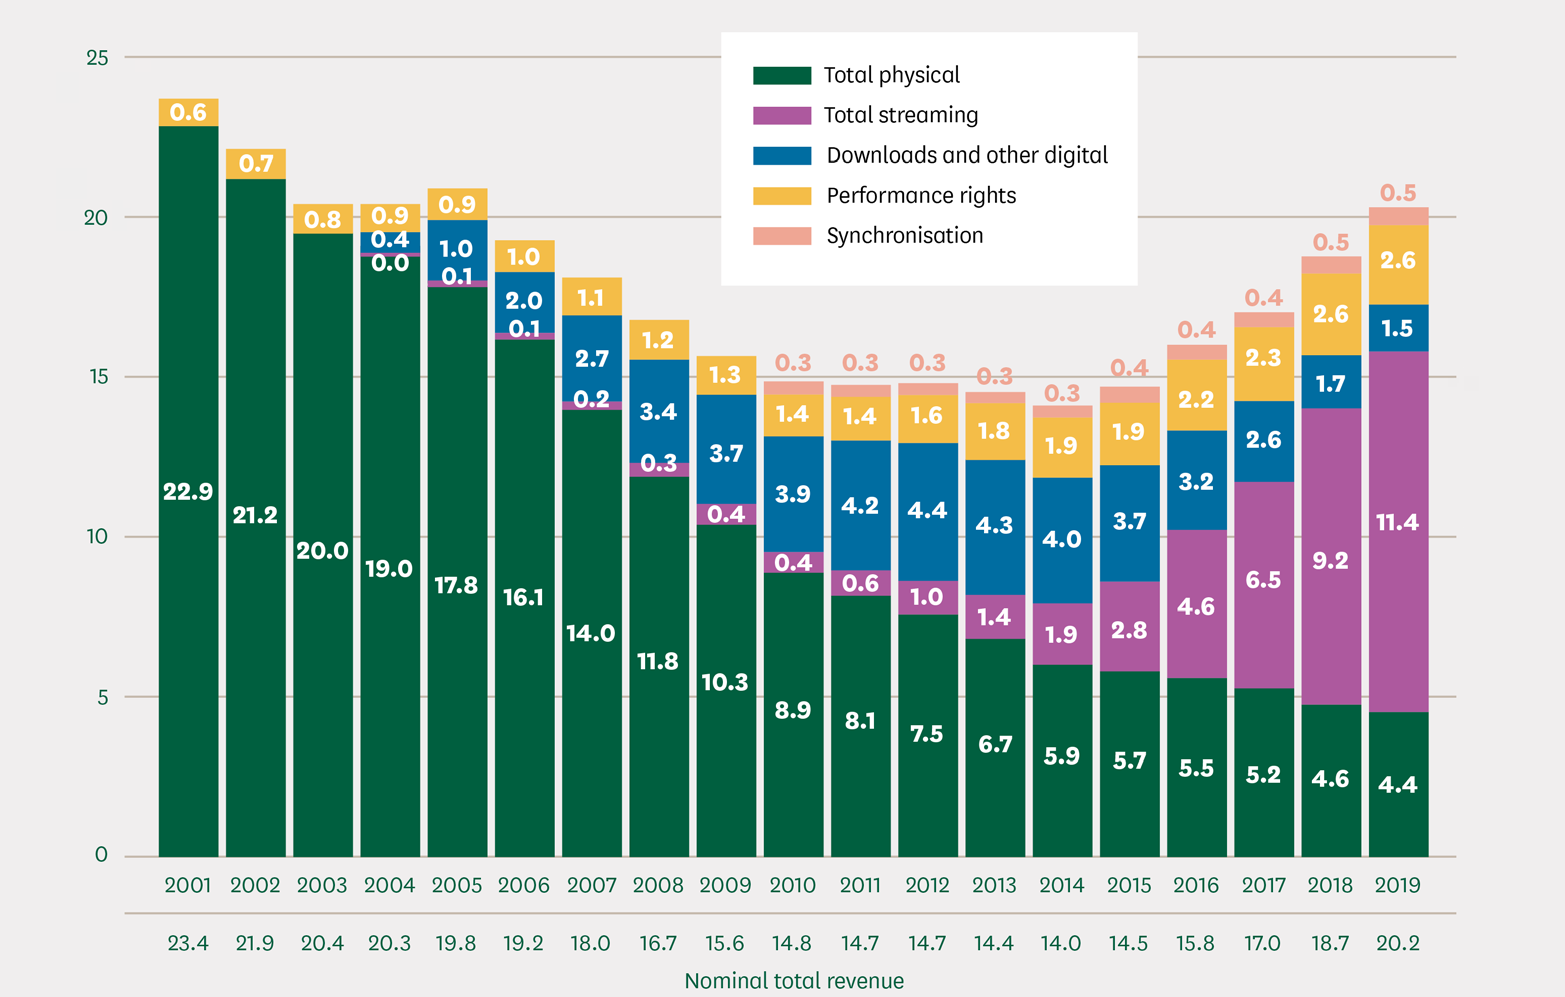
\includegraphics[width=1\linewidth]{img/receitas} \caption{Receita global da indústria da música (US\$ bi)}\label{fig:receitas}
\end{figure}

\hypertarget{caracterizauxe7uxe3o-teuxf3rica-do-setor-de-produuxe7uxe3o-de-bens-culturais}{%
\section{CARACTERIZAÇÃO TEÓRICA DO SETOR DE PRODUÇÃO DE BENS
CULTURAIS}\label{caracterizauxe7uxe3o-teuxf3rica-do-setor-de-produuxe7uxe3o-de-bens-culturais}}

Para caracterizar o setor de produção de bens culturais, nos muniremos
de \citet{bourdieu} e \citet{herscovici}. E, para que tal caracterização
seja coerente, deve-se manter, na medida do possível, um método e um
conjunto de conceitos coesos. Para tanto, analisaremos a seguir as
quatro hipóteses acerca do produto cultural adotadas por
\citet{herscovici}.

\hypertarget{hipuxf3tese-1}{%
\subsection{HIPÓTESE \#1}\label{hipuxf3tese-1}}

\begin{citacao}
Suponhamos que não seja possível raciocinar em termos de valor intrínseco da obra de arte. Isto significa simplesmente que as apreciações feitas a respeito da obra dependem, simultaneamente, da época e do grupo social considerado, assim como dos modos de validação em vigor. A obra só pode ser compreendida e apreciada se for recolocada no seu contexto histórico e sociológico; a universalidade da obra de arte é, portanto, limitada por estes fatores. \citep[p.~30]{herscovici}
\end{citacao}

Essa hipótese inviabiliza diretamente a caracterização do bem cultural
como mercadoria no conceito de Marx:

\begin{citacao}
O que determina a grandeza do valor, portanto, é a quantidade de trabalho socialmente necessária ou o tempo e trabalho socialmente necessário para a produção de um valor-de-uso. Cada mercadoria individual é considerada aqui um exemplar médio de sua espécie. [...] A grandeza do valor de uma mercadoria permaneceria, portanto, invariável, se fosse constante o tempo de trabalho para sua produção. \citep[p.~61]{marx}
\end{citacao}

Se o bem cultural não possui valor intrínseco, este não pode ser medido
pela quantidade de trabalho dispendida em seu processo de produção. Esse
tipo de bem, por outro lado, parece, à primeira vista, compatível com o
conceito de valor na teoria utilitarista:

\begin{citacao}
Ora, se há algum fato indiscutível sobre o valor de troca, é que ele não se refere de nehuma forma a um objeto, mas a uma circunstância de um objeto. Na verdade, o valor implica uma relação; mas se é assim, ele não pode ser \textit{alguma outra coisa}. Um estudante de Economia não poderá jamais ter esperança de alcançar idéias claras e corretas em sua ciência se conceber o valor de algum modo como uma \textit{coisa} ou um \textit{objeto}, ou mesmo como algo que esteja numa coisa ou objeto. As pessoas são assim levadas a falar de uma coisa não existente tal como \textit{valor intrínseco}. \citep[p.~66]{jevons}
\end{citacao}

\hypertarget{hipuxf3tese-2}{%
\subsection{HIPÓTESE \#2}\label{hipuxf3tese-2}}

\begin{citacao}
A atividade do produtor cultural, em relação ao jogo simbólico, deve aparece como "desinteressada": aparentemente, ela não corresponde a um comportamento econômico racional. Esta concepção, que vimos surgir desde o Renascimento, supõe a autonomia do campo cultural que aparece como um espaço social específico. Enfim, isso significa que o conjunto das racionalidades culturais se assemelha às racionalidades extra-econômicas, ou seja, a uma lógica dos fins. \citep[p.~31]{herscovici}
\end{citacao}

Tendo início por volta do século XV, a autonomização que o autor faz
referência passa, necessariamente, pela constituição da demanda de bens
simbólicos acima do ponto crítico em que profissionalização da atividade
de produção desse tipo de bem se torna viável. Com a revolução
industrial, essa formação é acelerada pela ``extensão do público
resultante da generalização do ensino elementar, capaz de permitir às
novas classes (e às mulheres) o acesso ao consumo cultural (por exemplo,
através da leitura de romances)'' \citep[p.~102]{bourdieu}.

Essas condições permitem ao campo intelectual e artístico a,
progessivamente, se libertar da tutela da ética e estética das
instâncias de legitimidade externas --- como a igreja e a corte ---, e
firmar suas próprias regras em uma tradição pautada na \emph{arte pela
arte}. Na medida que essa autonomia se desenvolve e se amplia, a classe
artística passa a exercer em suas esferas de legitimização um controle
exclusivo --- tanto no sentido de privado, restrito, quanto no sentido
de exclusão, pois cada vez mais exige o domínio de códigos de
comunicação progressivamente mais complexos ---, o que vai de encontro
às características da mercadoria no \emph{mainstream}.

A legitimização e avaliação de uma mercadoria no \emph{mainstream} é
definida pelo seu valor de uso e apreço --- sua utilidade total e
marginal, respectivamente --- e, principalmente, por sua escassez
\citep[p.~67-68]{jevons}. Em um ambiente concorrencial, esses elementos
determinarão também seu preço. Entretanto, um campo de produção de bens
culturais que visa exercer sua autonomia de forma exclusiva não pode ser
ao mesmo tempo legitimizado externamente pelas relações de troca da
mercadoria com o consumidor e nem pela utilidade de seus produtos
culturais, tornando evidente sua incompatibilidade teórica com o
\emph{mainstream}.

\hypertarget{hipuxf3tese-3}{%
\subsection{HIPÓTESE \#3}\label{hipuxf3tese-3}}

\begin{citacao}
Cada produto cultural aparece e é percebido como único. Mesmo quando produzido industrialmente, ele mantém as características de um produto único. Apesar do mecanismo de formação dos preços de mercado, seu valor de uso é único e aleatório. A personalização extrema dos modos de valorização desses produtos, ligada ao desenvolvimento e à exacerbação do "star-system", permite a organização e a manutenção desta escassex. \citep[p.~31]{herscovici}
\end{citacao}

Suponha que a utilidade de um indivíduo seja definida pela seguinte
função: \[U(x,y)=x^\alpha y^\beta\]

Para que esse resultado pudesser ter alguma coerência, deveríamos
aceitar que o consumo de dois bens culturais é melhor do que um.

Em que \(x\) represente a quantidade de bens culturais e \(y\) a
quantidade de outros bens. A dinâmica desse consumidor em relação aos
bens culturais pode ser entendida pela taxa de variação de sua
utilidade:
\[\frac{\frac{\partial U}{\partial x}}{U(x,y)} = \frac{\alpha x^{\alpha-1}y^\beta}{x^\alpha y^\beta} = \frac{\alpha}{x}\]

Esse resultado nos permitiria dizer que o consumo de mais um bem
cultural aumentaria a utilidade total do consumidor em
\(\frac{\alpha}{x}\).

\begin{itemize}
\tightlist
\item
  escrever hipóteses (livro Alain, p.30) (hipotese 1: falar da
  otimização (snyder p.~147), h2: Bourdieu, h3: homogeneidade e valor em
  Menger , h4: ?)
\item
  mostrar que a metodologia neoclássica não é capaz de caracterizar
  teoricamente os bens culturais:

  \begin{itemize}
  \tightlist
  \item
    função de produção, incluindo homogeneidade (p.27), utilidade
    ordinal x cardinal (impossibilidade somar utilidade ordinal) e star
    system
  \item
    leis de rendimentos marginais decrescentes
  \item
    função utilidade: consumo de duas músicas não é melhor do que de
    uma. Mostrar otimização restrita (renda e preços das músicas).
  \end{itemize}
\end{itemize}

\hypertarget{uma-teoria-pura-da-arte}{%
\subsection{UMA TEORIA PURA DA ARTE}\label{uma-teoria-pura-da-arte}}

A análise das hipóteses trazidas por \citet{herscovici} nos permite
supor que, por conta das características do produto cultural, o
\emph{mainstream} seja inadequado para situar metodologicamente uma
análise do setor de produção desses bens e, por consequência, deve-se
buscar uma alternativa. Bourdieu propõe uma \emph{teoria pura da arte},
que trate da dualidade do produto cultural como valor puramente
simbólico e como mercadoria:

\begin{citacao}
[...] tudo leva a crer que a constituição da obra de arte como mercadoria e a aparição, devido aos progressos da divisão do trabalho, de uma categoria particular de produtores de bens simbólicos especificamente destinados ao mercado, propiciaram condições favoráveis a uma teoria pura da arte --- da arte como tal ---, instaurando uma dissociação entre a arte como simples mercadoria e a arte como pura significação, cisão produzida por uma intenção meramente simbólica e destinada à apropriação simbólica, isto é, a fruição desinteressada e irredutível à mera posse material. \citep[p.~103]{bourdieu}
\end{citacao}

O bem cultural pode, nessa concepção, ter ao mesmo tempo valor
simbólico, ou seja, ser \emph{arte}, e não estar ofertado no mercado, de
forma que não seja \emph{mercadoria}. Entretanto, enquanto mercadoria
ele não deixa de ser arte, independentemente do quanto é sua
legitimidade dentre a classe artística. Isso porque o valor simbólico do
bem cultural depende da percepção do produtor ou do observador, que
varia de acordo com o contexto social e histórico. Uma vez percebido
como arte, o será \citep[p.~272]{bourdieu}.

\begin{itemize}
\tightlist
\item
  Tratar do setor de produção erudito e popular
\end{itemize}

\hypertarget{tese}{%
\section{TESE}\label{tese}}

\begin{enumerate}
\def\labelenumi{\arabic{enumi}.}
\tightlist
\item
  Com redução de receitas, fortalecimento do star system, causando
  oligopolização da indústria cultural;
\end{enumerate}

\renewcommand\refname{REFERÊNCIAS}
  \bibliography{bib.bib}

\end{document}
